


\textbf{Erster Feldversuch}
\label{ersterFeldVer}

Im ersten Versuch wurde untersucht, wie sich die Andruckzeit des Tapes auf das Messergebnis auswirkt. Bereits nach 5 Sekunden war ein Ergebnis messbar, welches bei 120 Sekunden ausgeprägter wurde.

\begin{figure}[H]
    \centering
    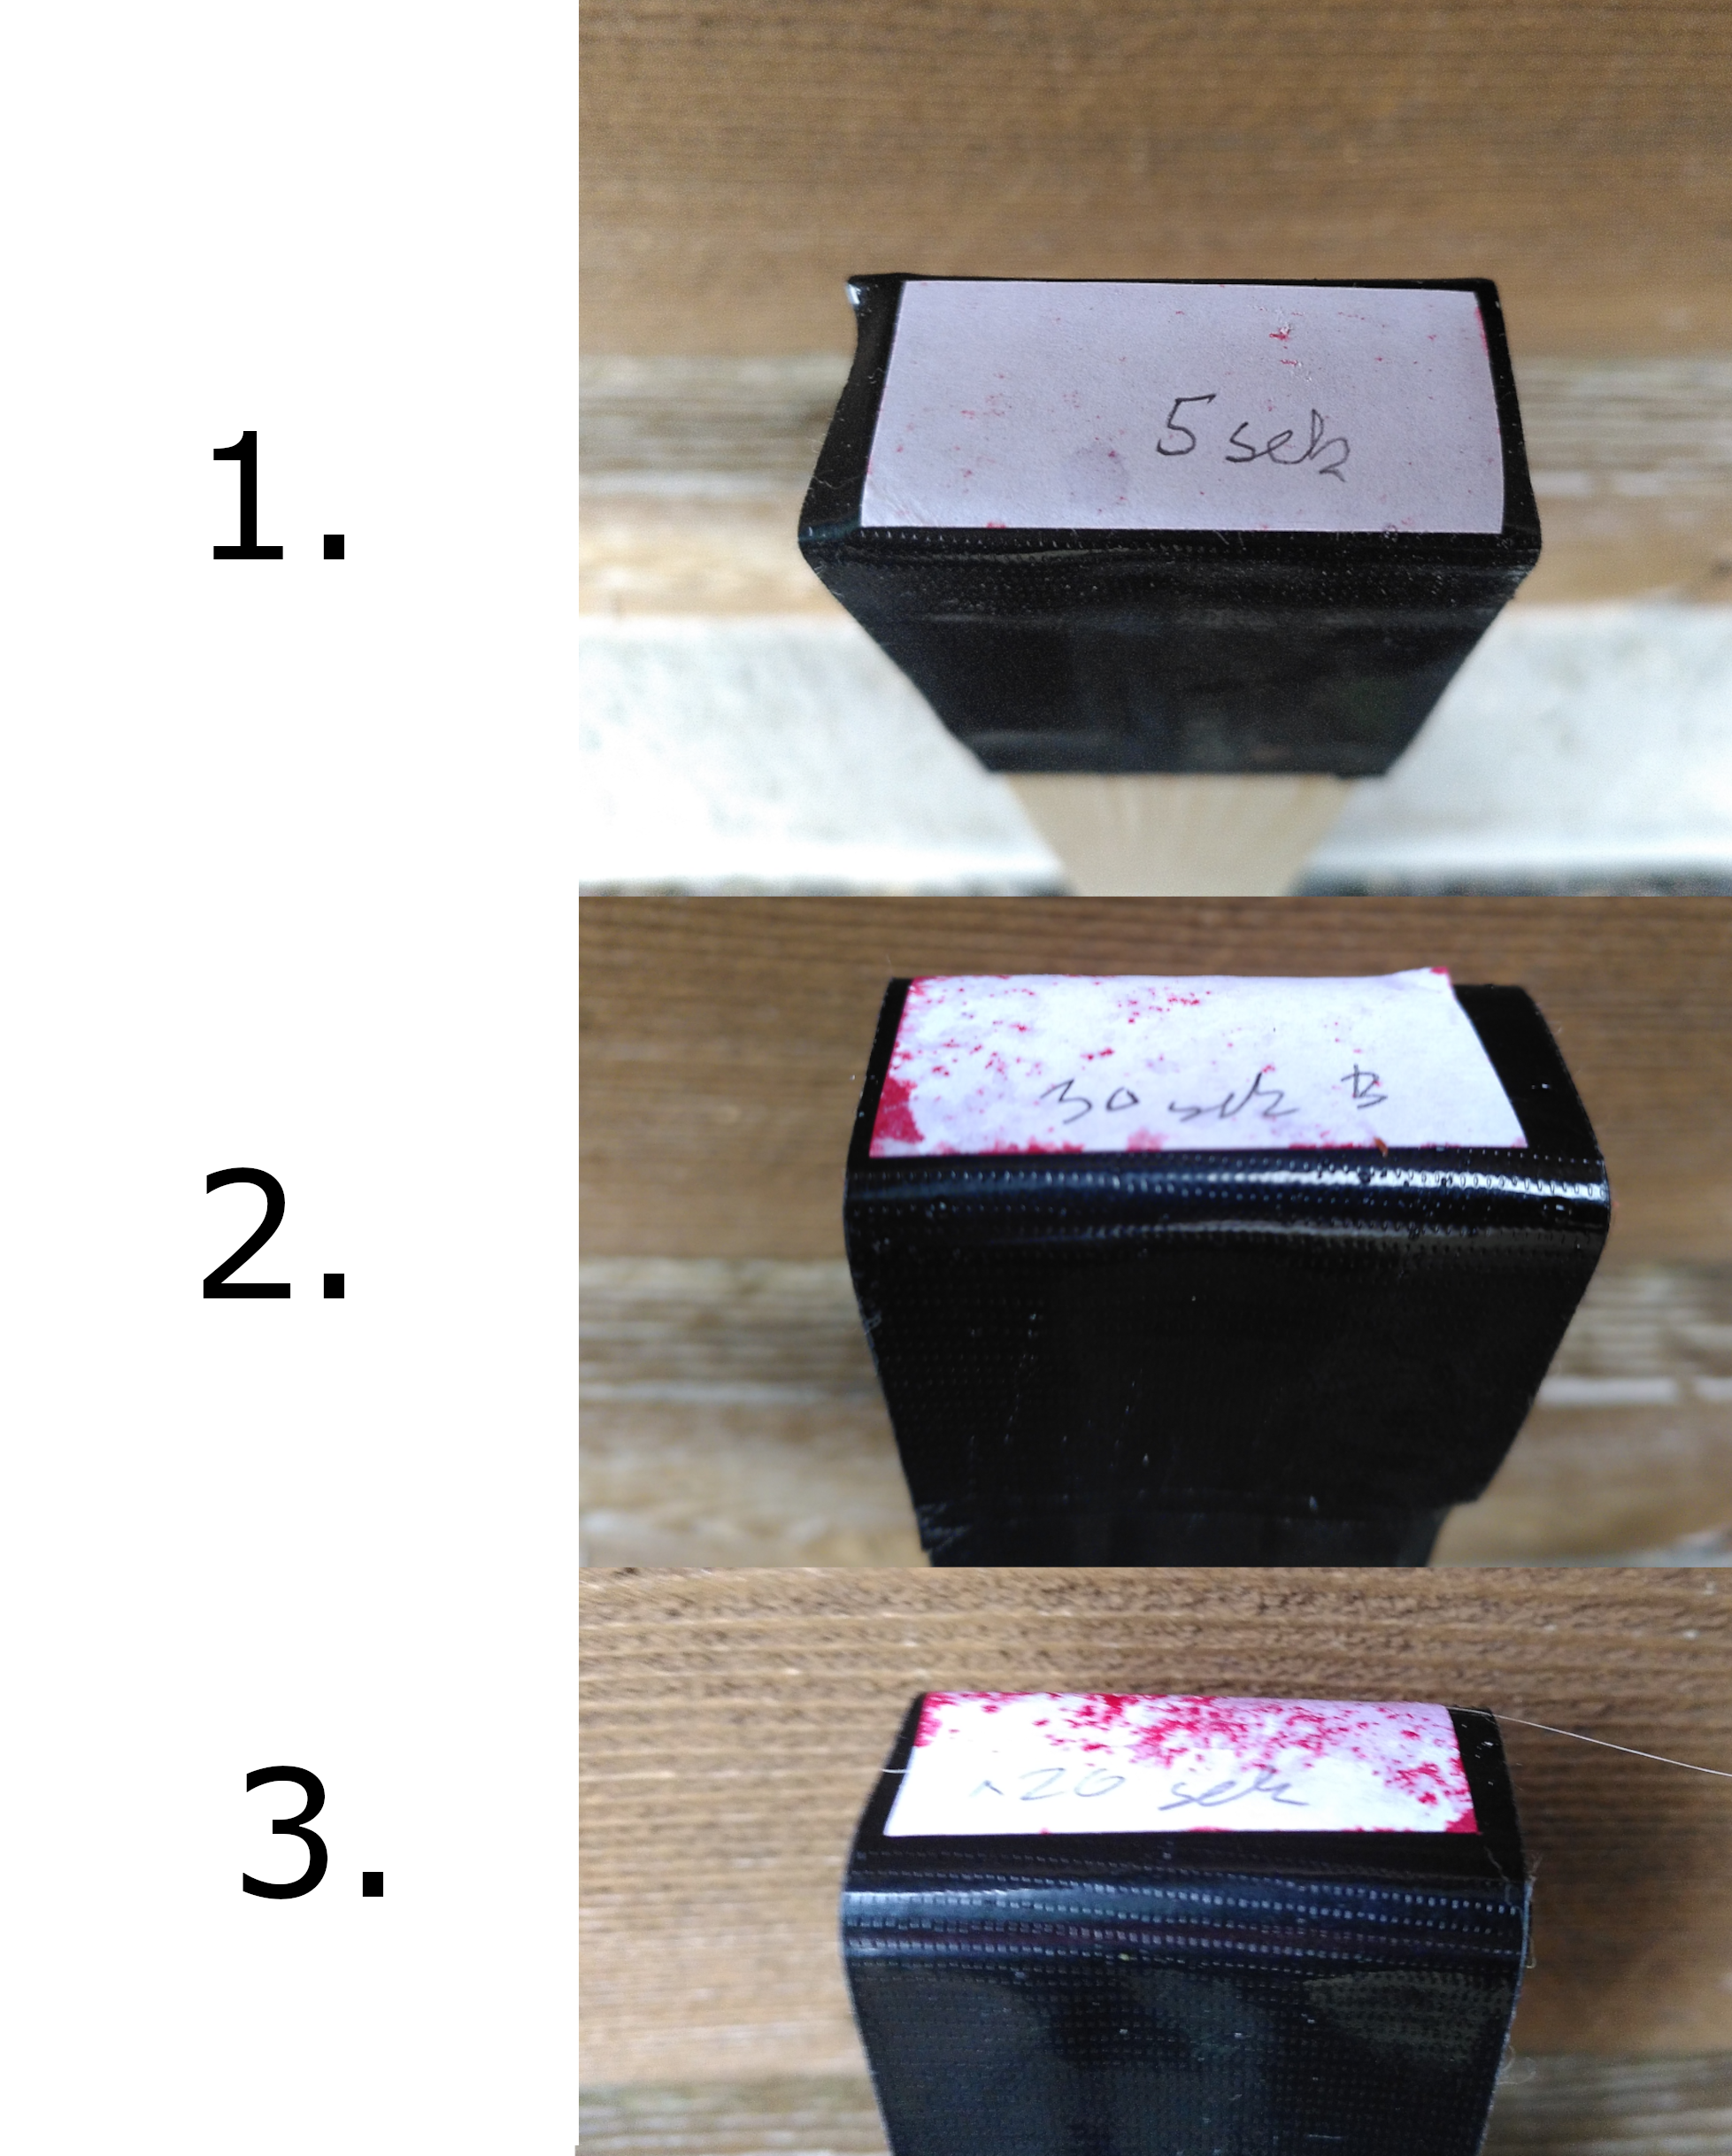
\includegraphics[width=0.8\textwidth]{Bilder/ZeitAbha.png}
    \caption{Drei Tapes gemessen bei nassem Schnee, da es geregnet hat: 1. 5 Sekunden Anpresszeit, 2. 30 Sekunden Anpresszeit, 3. 120 Sekunden Anpresszeit} 
    \label{fig:ZeitDruck}
\end{figure}

\newpage
\textbf{Zweiter Feldversuch}
\label{zweitFeldVer}
Ziel des zweiten Versuchs \ref{fig:DavosMessung} war es, den Ablauf der Tape-Messung bei verschiedenen LWC-Werten zu testen. Dazu wurde Schnee einmal mit Wasser übergossen und einmal mit Kältespray eingefroren. Die Ergebnisse sind in \ref{fig:DavosMessungErg} dargestellt. Die Wärmebildaufnahme \ref{fig:KaltSchnee} zeigte, dass der Schnee nur lokale Terperaturänderung macht, da Schnee gut isoliert. 

\begin{figure}[H]
    \centering
    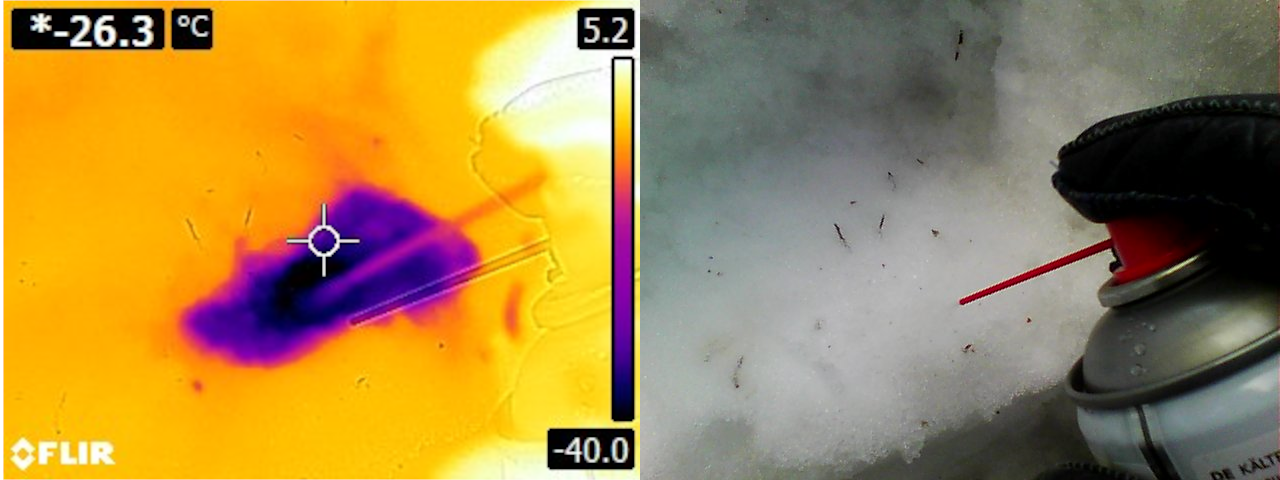
\includegraphics[width=0.8\textwidth]{Bilder/KalterSchnee.png}
    \caption{Wärmebildaufnahme der gekühlten Schneestelle, welche zur Simulation eines niedrigen LWC verwendet wurde.} 
    \label{fig:KaltSchnee}
\end{figure}



\begin{figure}[H]
    \centering
    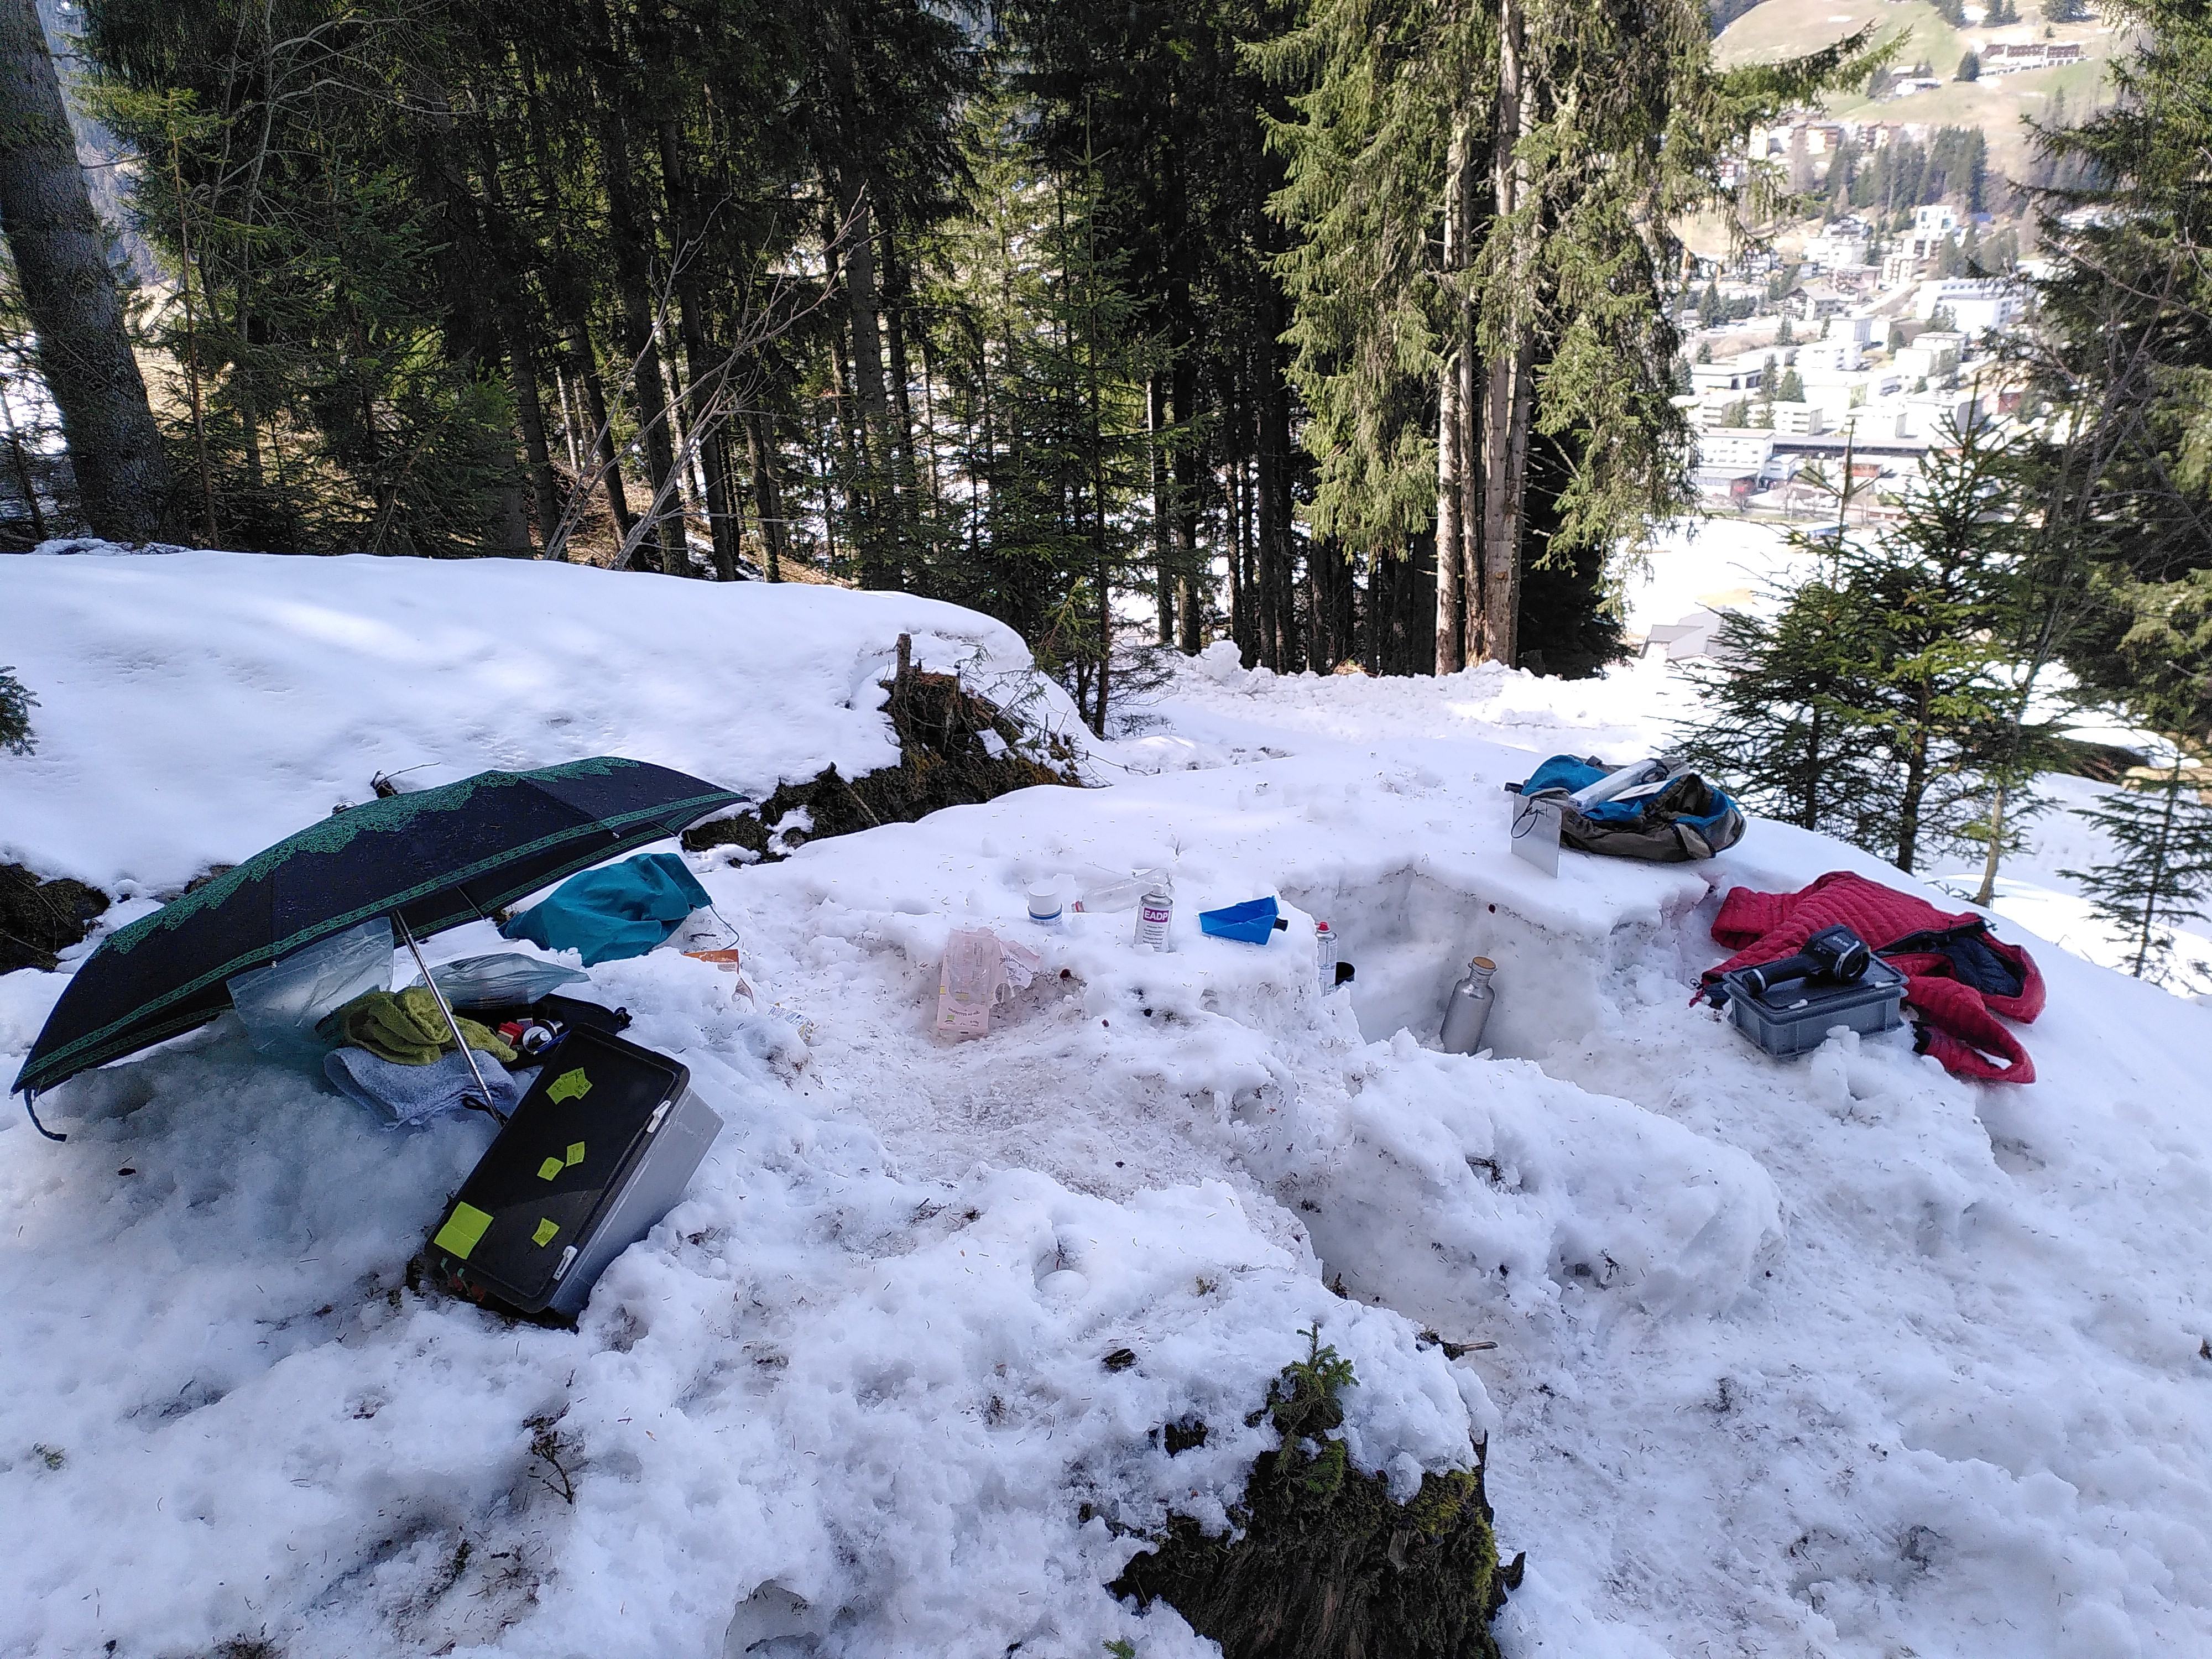
\includegraphics[width=0.8\textwidth]{Bilder/IMG_20240411_124421.jpg}
    \caption{Messstandort in Davos, unter dem Regenschirm ist das Tape gelagert, um es vor direkter Sonneneinstrahlung und Wasser Tropfen zu schützen.} 
    \label{fig:DavosMessung}
\end{figure}

\begin{figure}[H]
    \centering
    \includegraphics[width=0.8\textwidth]{Bilder/UnterschiedlicheLWC.png}
    \caption{Tapes aus dem ersten Feldversuch: 1. Unveränderter Schnee, 2. Gekühlter Schnee (siehe Abb. \ref{fig:KaltSchnee}),  3. Mit flüssigem Wasser übergossener Schnee.} 
    \label{fig:DavosMessungErg}
\end{figure}


%\caption{Ein bild von 'normalem' schnee}
\newpage


\label{drittFeldVer}

\begin{figure}[H]
    \centering
    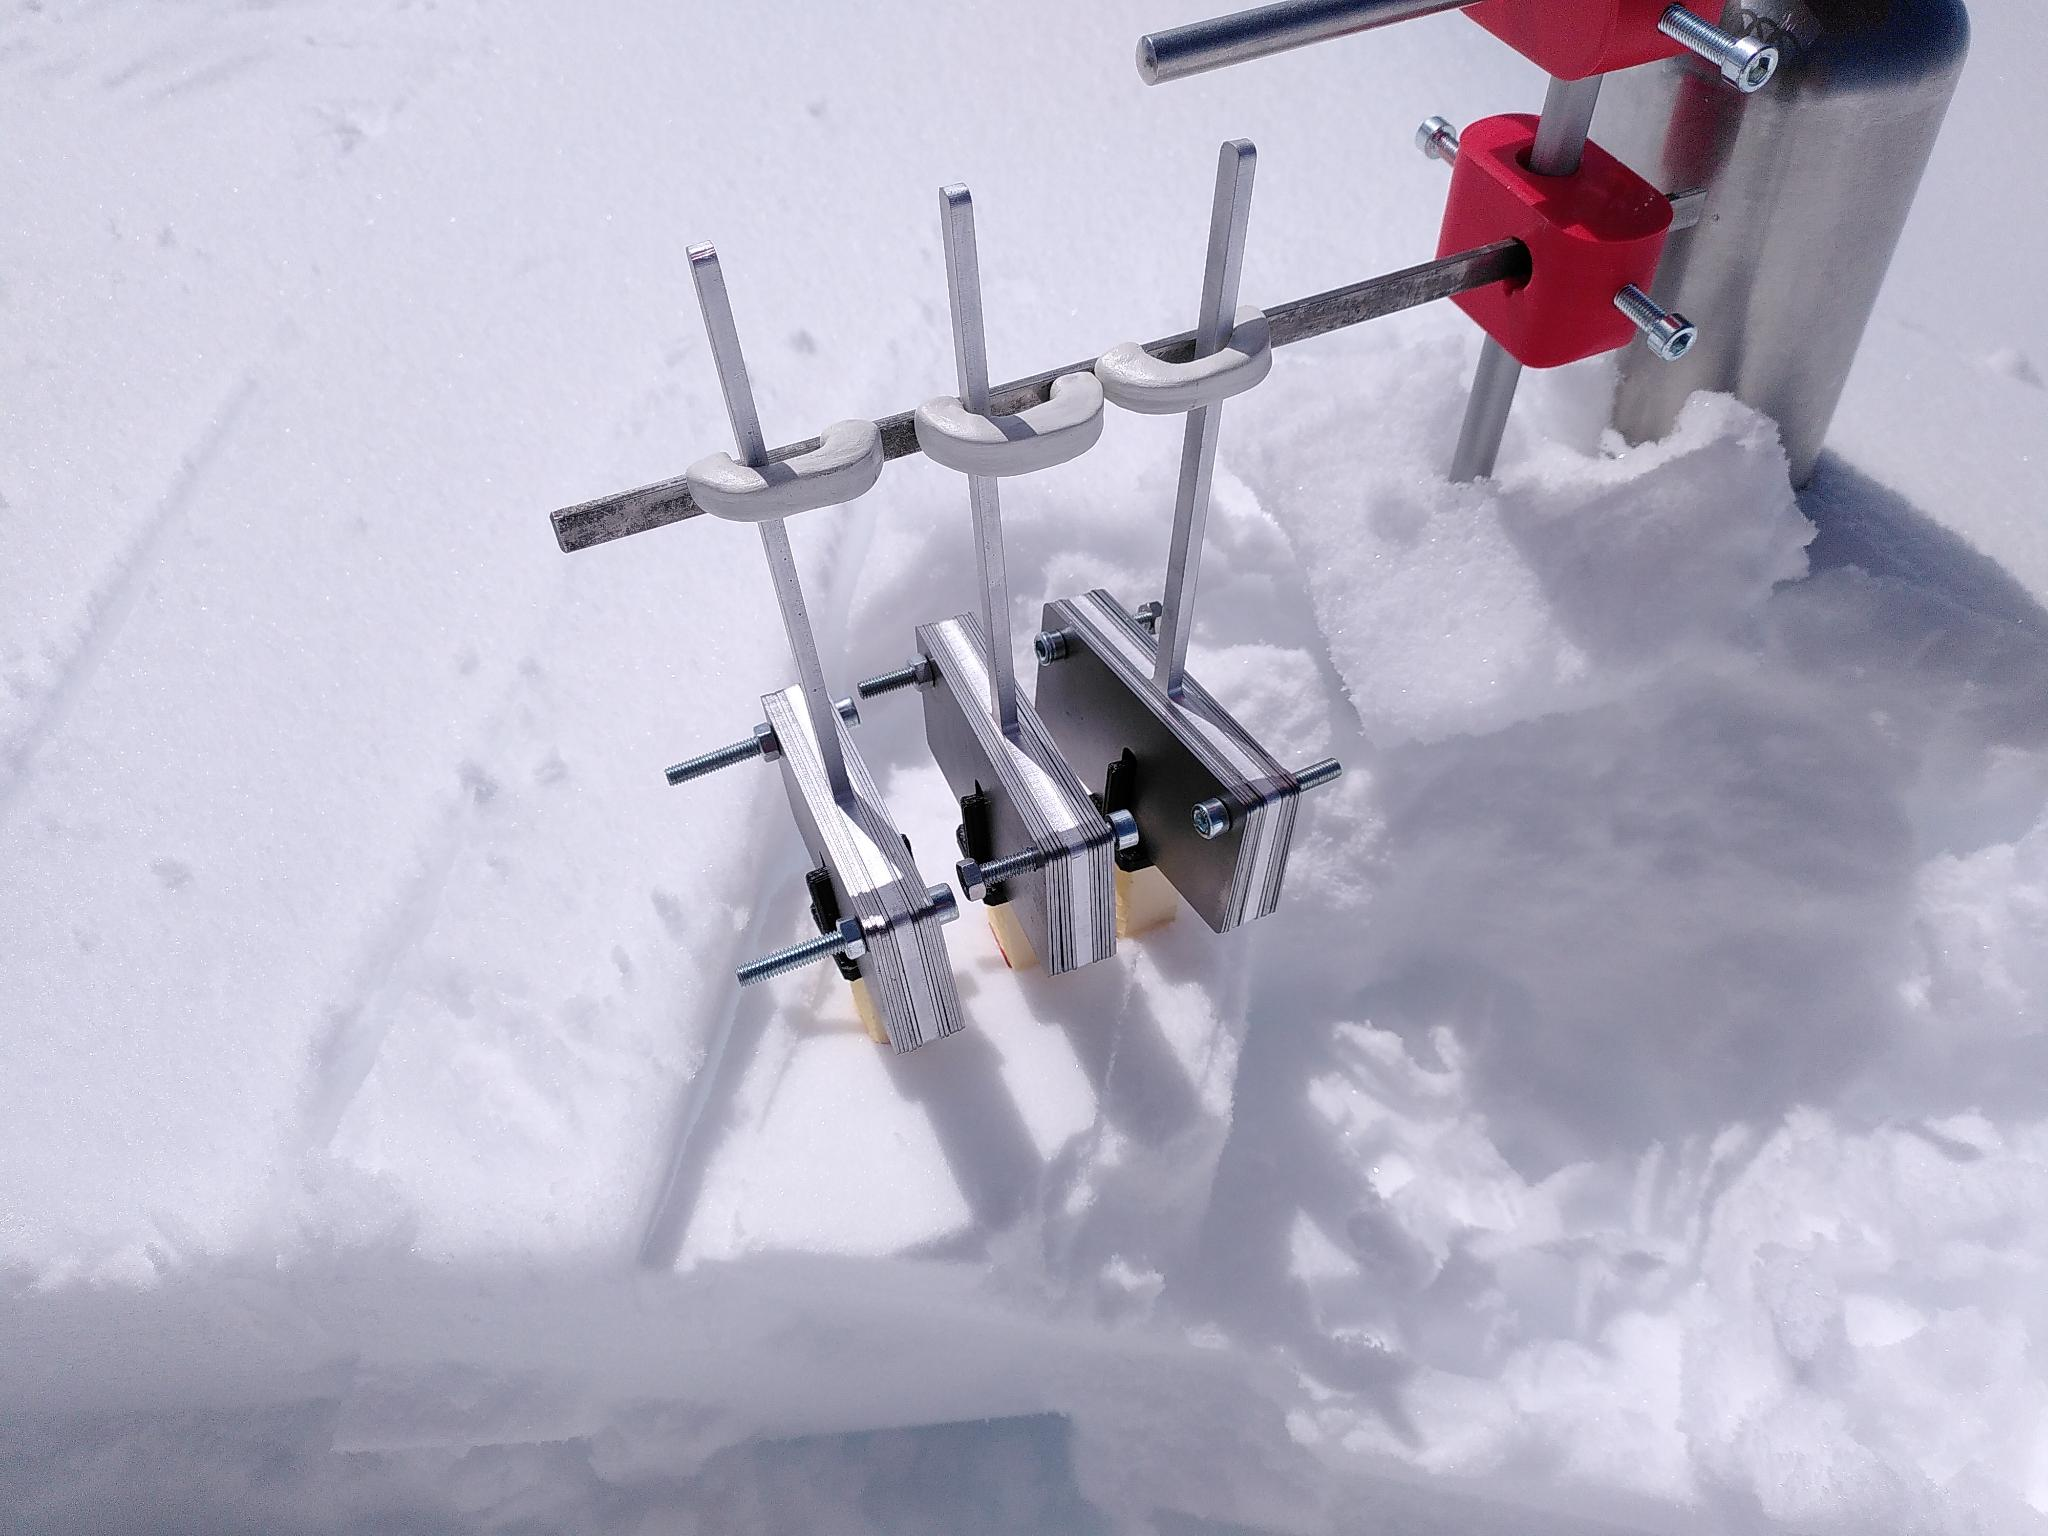
\includegraphics[width=0.8\textwidth]{Bilder/aufbauTitlis.jpeg}
    \caption{Messaufbau von drei Tapes auf unverändertem Schnee} 
    \label{fig:aufbauTitlis}
\end{figure}
\textbf{dritter Feldversuch}
Im dritten Versuch \ref{fig:aufbauTitlis} wurde ein neues Design mit variablem Anpressdruck getestet. Es zeigte sich, dass die Varianz der Tapes am geringsten war, wenn das Gewicht 80\% der maximalen Tragkraft des Schnees betrug. In \ref{fig:12Palt} ist das Ergebnis zu sehen.

\begin{figure}[H]
    \centering
    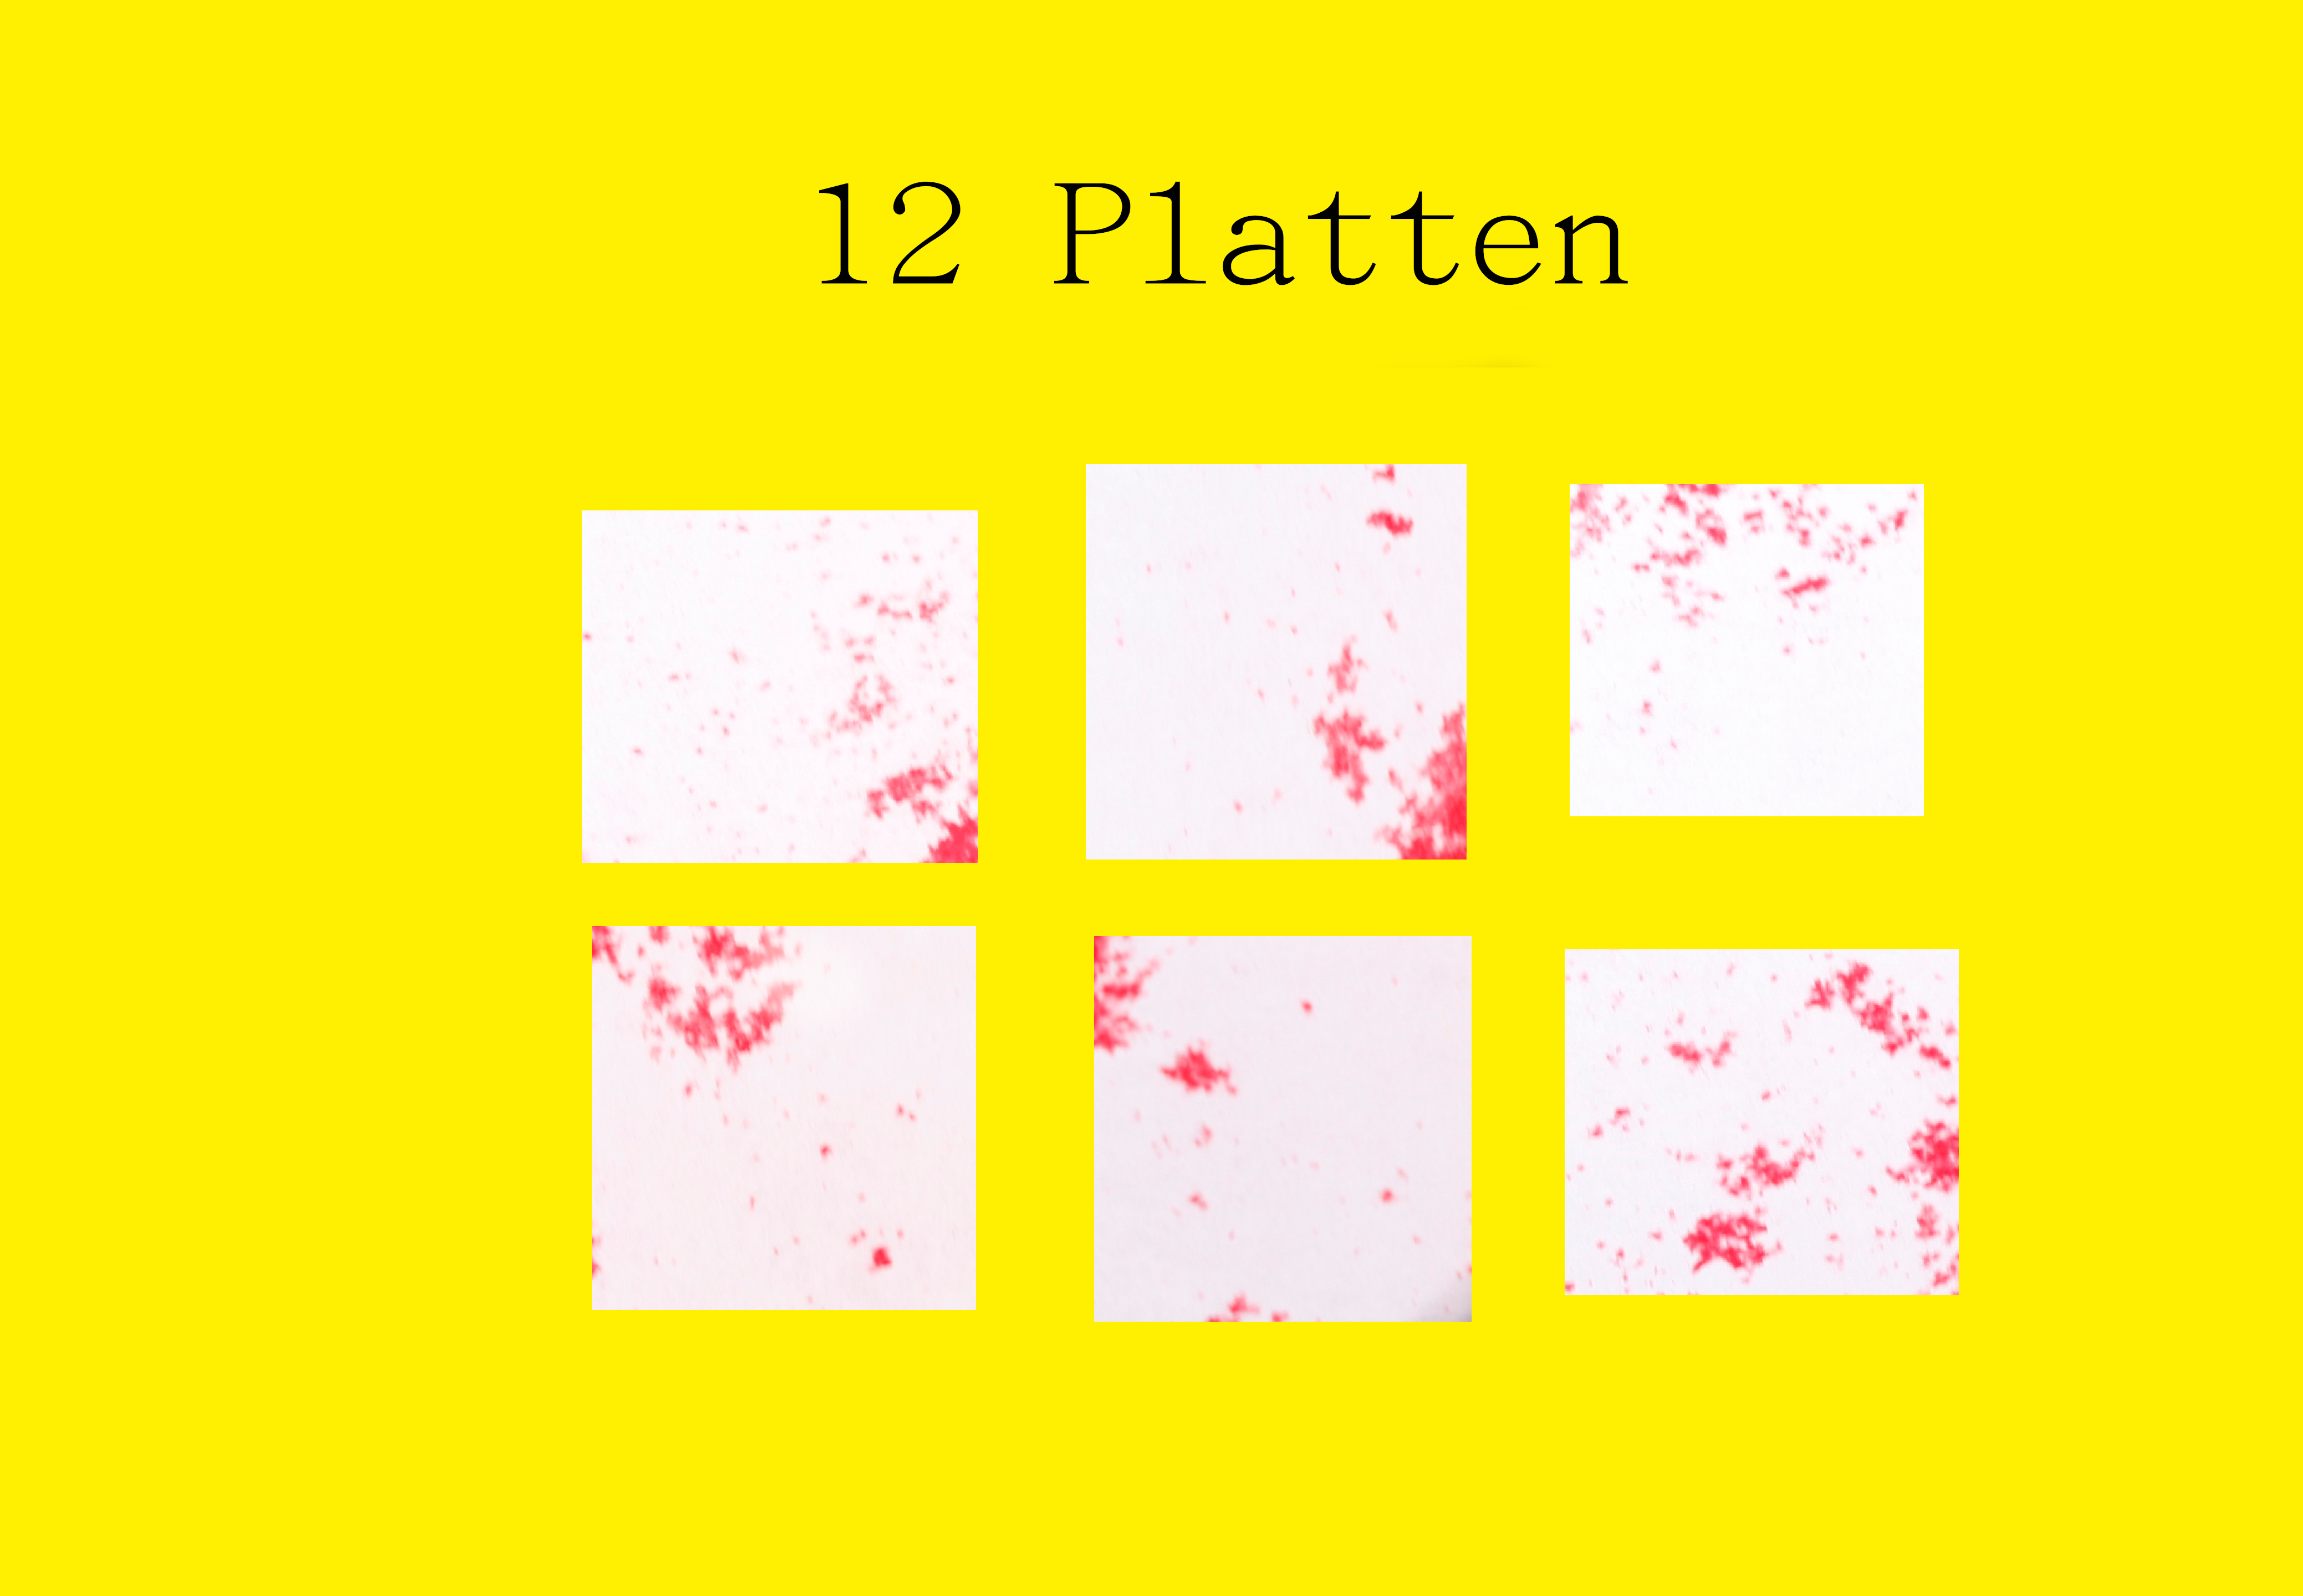
\includegraphics[width=0.8\textwidth]{Bilder/12Platten.png}
    \caption{Messung von sechs Tapes mit  zwölf Stahlplatten und einem Gesamtgewicht von 514 g auf unverändertem Schnee, um die Varianz der Messergebnisse zu bestimmen.} 
    \label{fig:12Palt}
\end{figure}

\newpage
Es wurde auch untersucht, wie sich das Tape verhält, wenn derselbe Schnee mehrmals hintereinander getestet wird. Dabei zeigte sich, dass die Menge an Wasser, die benötigt wird, um das Tape zu befeuchten, während der 120 Sekunden Andruckzeit vom Schnee bereitgestellt werden kann. Im Feldversuch wurde die Messung sechs mal wiederholt. \ref{fig:aufbauTitlis}


\begin{figure}[H]
    \centering
    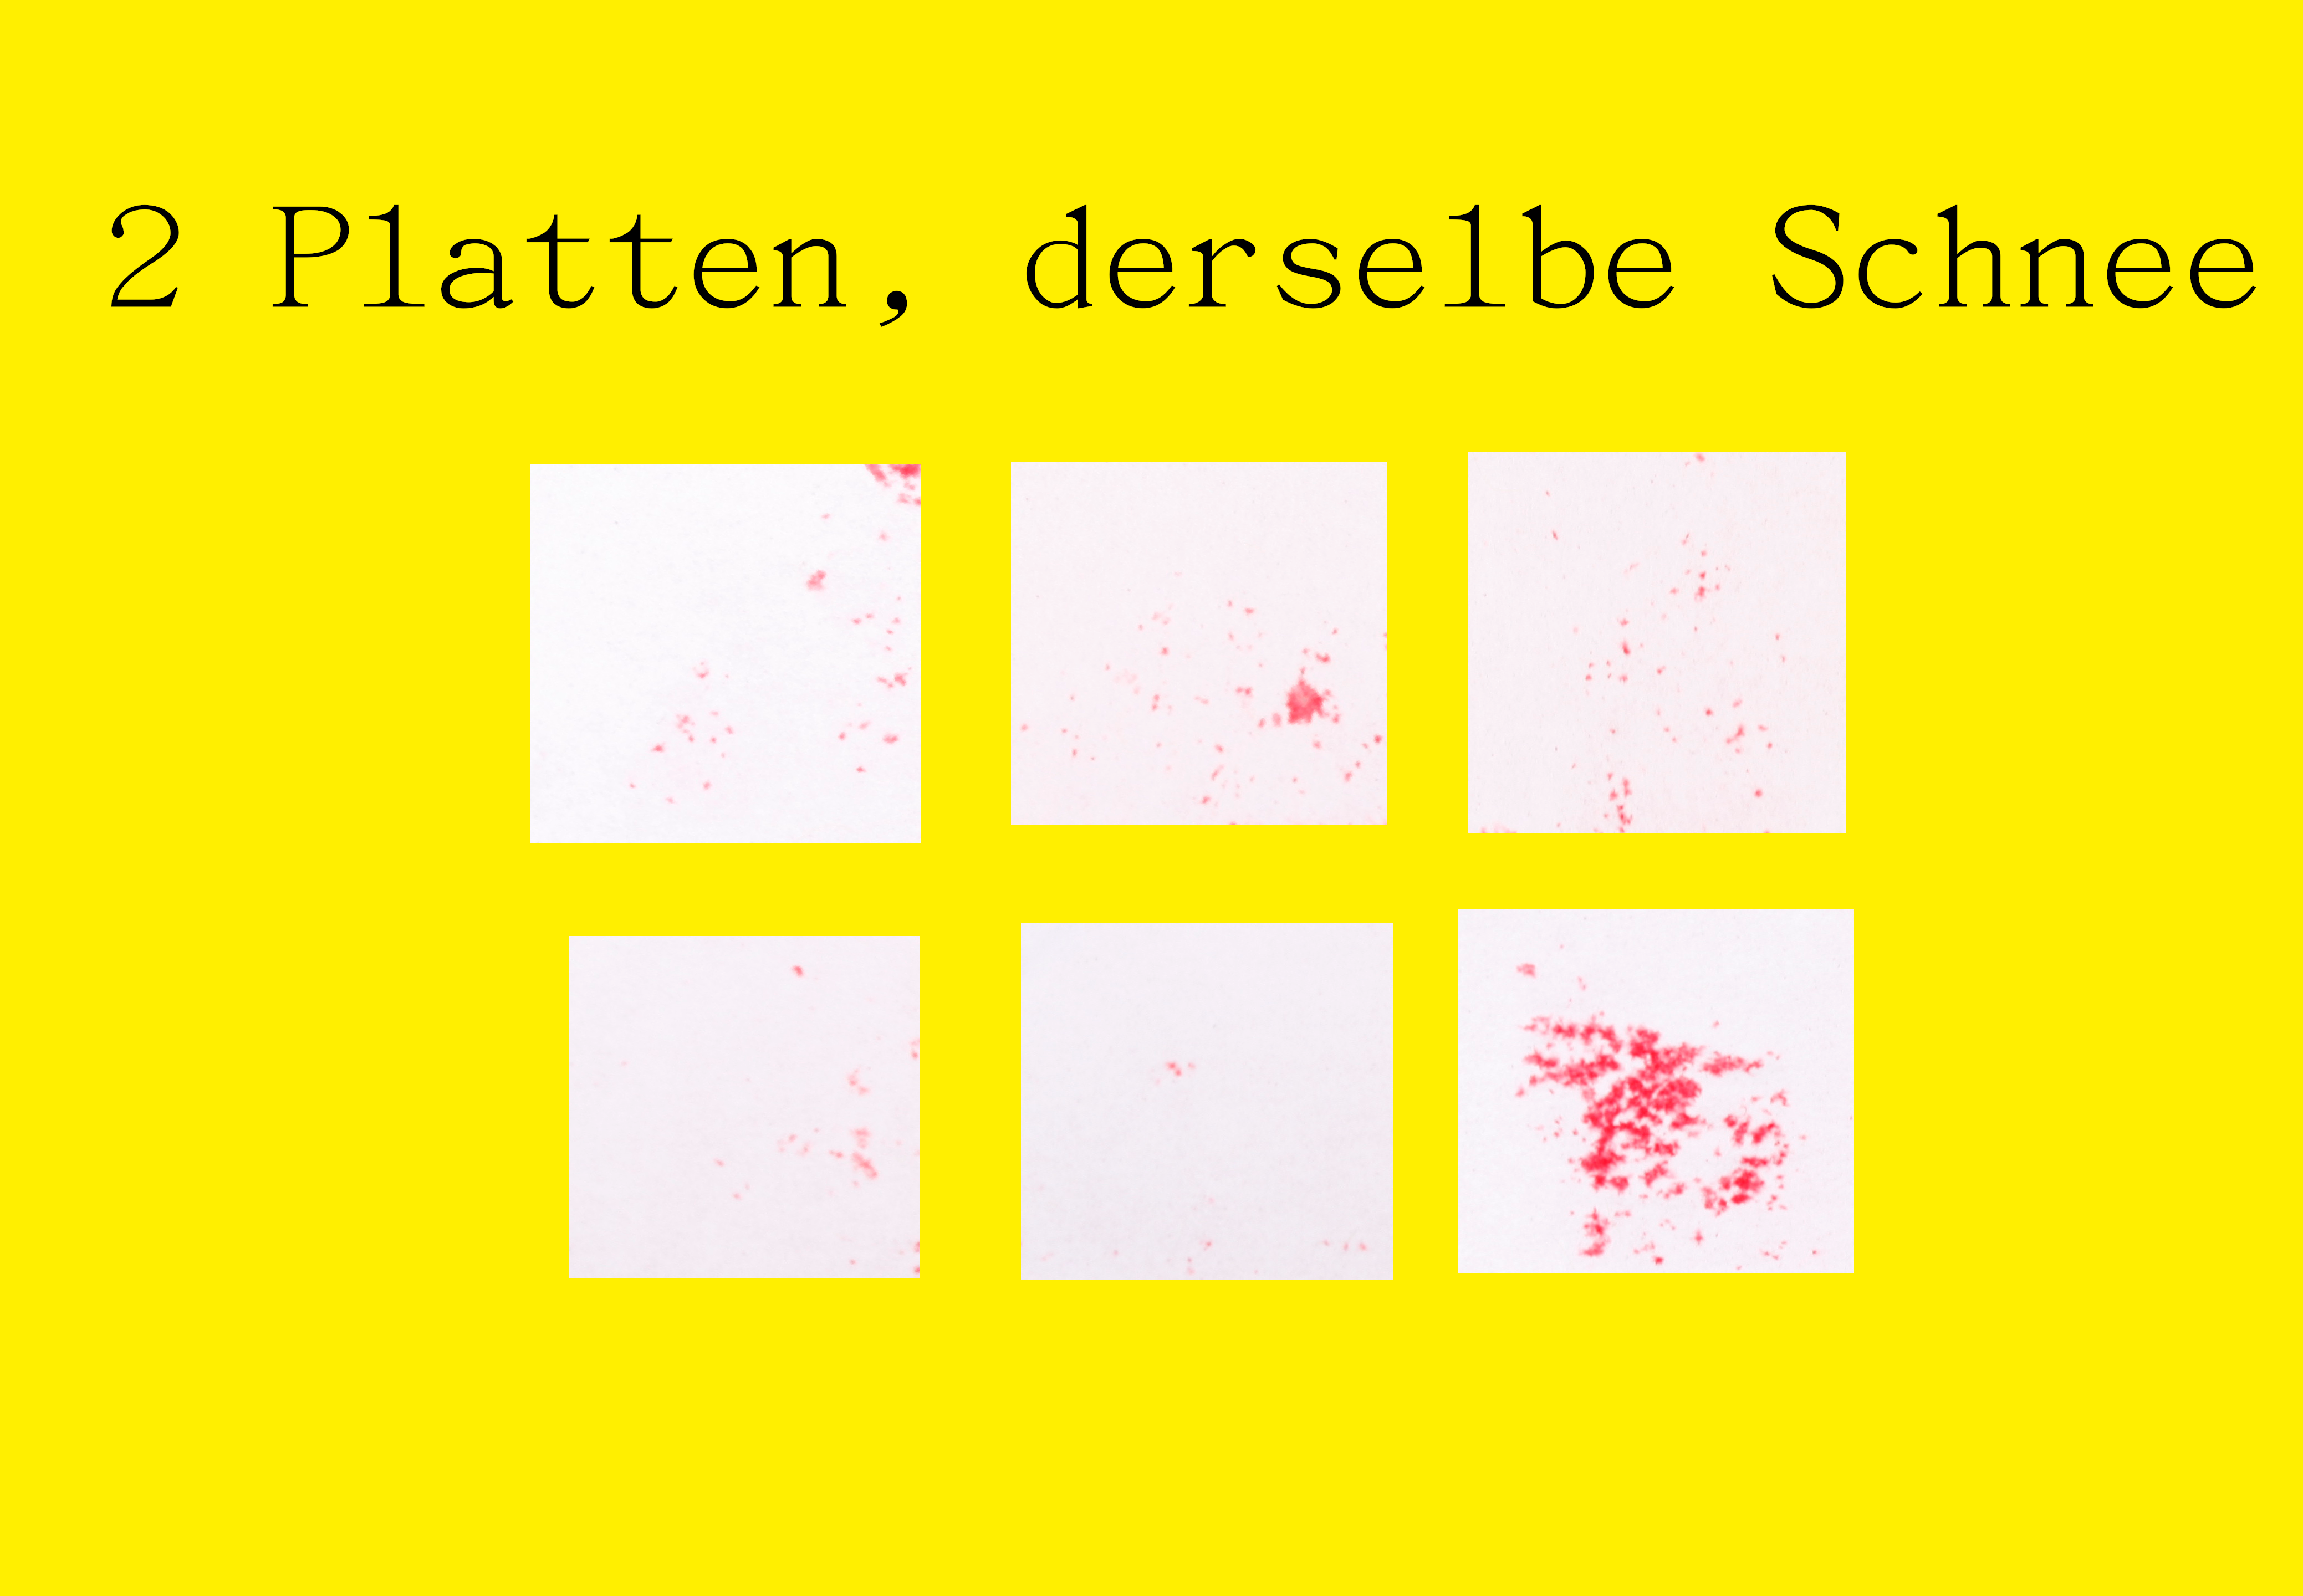
\includegraphics[width=0.8\textwidth]{Bilder/2PlattenSelberSchnee.png}
    \caption{Messung von sechs Tapes auf dem selben unverändertem Schnee, um die Einflüsse des Messen auf den Schnee zu erkennen.} 
    \label{fig:aufbauTitlis}
\end{figure}
